\chapter{Application Flow Monitoring}

\begin{chapintro}

Deep packet inspection (DPI) and basic flow monitoring are frequently used network monitoring approaches nowadays. Although the DPI provides application visibility, detailed examination of every packet is computationally intensive to be performed on high-speed networks. The basic flow monitoring achieves high performance by processing only packet headers but provides no details about the traffic content. Application flow monitoring is proposed as an attempt to combine DPI accuracy and basic flow monitoring performance. The aim of this chapter is to provide a complete information about application flow monitoring. 

The contribution of this chapter is threefold. Firstly, it provides an overview of the current state of application flow monitoring. Secondly, it defines consistent terminology and provides a workable definition of application flow and application flow record. The third contribution is an experimental study of an HTTP parser design. Despite extensive work, flow exporters generally fall short of performance goals due to extracting application layer data. Constructing effective protocol parser for in-depth analysis is a challenging and error-prone affair. We designed and evaluated several HTTP protocol parsers representing current state-of-the-art approaches used in today's flow exporters. We show the packet rates achieved by respective parsers, including the throughput decrease (performance implications of application parser) which is of the utmost importance for high-speed deployments. The presented results provide researchers and network operators with important insight into application flow monitoring deployment performance.


% Petr Velan and Pavel Čeleda. “Next Generation Application-Aware Flow Monitoring” - related but cannot be directly included.
% Petr Velan, Tomáš Jirsík, and Pavel Čeleda. “Design and Evaluation of HTTP Protocol Parsers for IPFIX Measurement”
The papers related to this chapter are~\cite{Velan-2014-Next, Velan-2013-Design}.
%The paper~\cite{Velan-2014-Next} is also relevant to this chapter, but its content was not directly included.

The organisation of this chapter is as follows:
\begin{itemize}
  \item Section~\ref{sec:app-motivation} provides motivation for processing the application layer in the flow monitoring.
  \item Section~\ref{sec:app-rel-work} outlines the state of the art in the field of application flow monitoring.
  \item Section~\ref{sec:app-flow-definition} defines necessary terminology and provides a definition of application flow and application flow record.
  \item Section~\ref{sec:creating-application-flow} describes how the application layer processing affects the flow monitoring.
  \item Section~\ref{sec:http-parser-design} is a case study of an HTTP parser design and of the effect of processing the HTTP protocol on the flow monitoring process.
  \item Section~\ref{sec:app-summary} summarizes the chapter.
\end{itemize}

\end{chapintro}

\newpage


\section{Motivation}\label{sec:app-motivation}

The number of different applications communicating over the Internet is ever increasing and so is the need for application-aware network monitoring. However, building network monitoring systems is always a compromise between accuracy and performance. The more detailed the information processing, the more accurate the monitoring system is. Unfortunately, a thorough examination of the traffic is computationally expensive~\cite{Gao-2006-Efficient, Lai-2004-Parallel}. Application flow monitoring is a network monitoring approach created to exploit the benefits of deep packet inspection (DPI). Integration of the DPI into flow monitoring allows for information aggregation, which provides better performance than the DPI alone.

Application flow monitoring is a subset of flow monitoring as described in the Chapter~\ref{chap:network-flow-monitoring} and all provided definitions hold for it as well. The reason to treat application flow monitoring as a special case is that processing application layer introduces specific issues which require special attention. Therefore, we distinguish basic flow monitoring (flow keys and values of other properties are extracted only from link, network, and transport layer headers) and application flow monitoring as two distinct part of flow monitoring.

The application flow monitoring usually utilizes two main concepts: application identification (also known as traffic classification) and application visibility. A complete definition of application flow monitoring is provided in Section~\ref{sec:app-flow-definition}. The application identification allows recognizing the application protocol of a particular flow. The type of application is usually added as a single field to the exported flow record. The application visibility provides more information about the information carried by the application protocol itself. Application identification is a prerequisite of the application visibility. However, application identification can be performed with use of machine learning techniques even without observing packet payloads.

This chapter describes the differences between basic flow monitoring and application flow monitoring that have to be taken into consideration when the application flow monitoring process is designed and deployed. The most important part of application visibility is the design of application parsers. To illustrate the complexity of the application parser design, we propose and discuss several designs of HTTP protocol parsers at the end of this chapter.

The benefits of application flow monitoring are discussed extensively in Chapter~\ref{chap:traffic-analysis-using-application-flow-monitoring}.

\section{Related Work}\label{sec:app-rel-work}

% TODO: https://tools.ietf.org/html/rfc6759#section-7.1.2
% https://www.cisco.com/c/en/us/td/docs/ios-xml/ios/qos_nbar/prot_lib/config_library/nbar-prot-pack-library.html
% honza bariancik HTTP v cisco
% CISCO Encrypted Traffic Analytics (ETA) - informace z TLS hlavicek

The use of machine learning techniques for traffic classification has attracted many researchers~\cite{Nguyen-2008-Survey, Dainotti-2012-Issues, Finsterbusch-2014-Survey}. A complete survey of the used techniques and results is out of the scope of this work, however, the methods of application identification in encrypted traffic are surveyed in Chapter~\ref{chap:measurement-of-encrypted-traffic}.

\subsection{Application Parsers}
Although application visibility is provided by a variety of commercial products such as dedicated probes, forwarding devices, and firewalls, it does not seem to be as attractive research topic as application identification where various machine learning and pattern matching algorithms can be applied. However, a significant research effort was invested in automating the creation of application parsers. \citeauthor{Pang-2006-binpac} created a language and accompanying parser called \emph{binpac}~\cite{Pang-2006-binpac} in \citeyear{Pang-2006-binpac}. It allows generating application parsers from their declarative description. A slightly different approach was taken by \citeauthor{Caballero-2007-Polyglot} in \citeyear{Caballero-2007-Polyglot}. The authors created a tool called \emph{Polygot}~\cite{Caballero-2007-Polyglot} which is used to reverse engineer application protocol headers. Similar work was published at the same time by \citeauthor{Cui-2007-Discoverer} in \cite{Cui-2007-Discoverer}. They presented a tool called \emph{Discoverer} that could automatically reverse engineering the protocol message formats of an application from its network trace. \citeauthor{Davidson-2009-Protocol} introduce a notion of using a higher order attribute grammar in~\cite{Davidson-2009-Protocol}, which allows describing the structure of application protocols for which the use of context-free grammar is impractical or impossible. Another framework, called \emph{Spicy}~\cite{Sommer-2016-Spicy} was introduced by \citeauthor{Sommer-2016-Spicy}. It consists of a format specification language, compiler toolchain and an API for DPI applications which allows for easy integration of the generated parsers to existing tools.

\subsection{Application Flow Exporters}
There is a number of open-source tools and commercial products that support an export of flows including application level information. Most of them already support the IPFIX protocol for the encoding of application information~\cite{Hofstede-2014-Flow}, however, there are still a few that add custom elements to the NetFlow v9 protocol, which can cause element collisions and compatibility problems. Table~\ref{tab:flow-exporters} shows an overview of the flow exporters discussed in this section.

\begin{table}[ht!]
    \centering
    \footnotesize
    \renewcommand{\arraystretch}{1.2}
    \begin{tabular}{>{\centering}m{1.5cm}| >{\centering}m{2cm} |c|>{\centering}m{0.8cm}|>{\centering\arraybackslash}m{6.0cm}}
    \toprule
    \textbf{Vendor}    & \textbf{Product}                   & \textbf{IPFIX} & \textbf{App. ident.} & \textbf{App. visibility}  \\ \hline
    CERT NetSA         & YAF                                & \cmark         & \cmark                       & FTP, HTTP, IMAP, RTSP, SIP, SMTP, SSH, DNS, SSL/TLS, IRC, NNTP, POP3, SLP, TFTP, MySQL, DNP3, Modbus and RTP \\ \hline
    ntop               & nProbe                             & \cmark         & \cmark                       & \\ \hline
    ntop               & nProbe Pro                         & \cmark         & \cmark                       & HTTP, DHCP, DNS, MySQL, Oracle DB, BGP, IMAP, POP3, SMTP, Radius, Diameter, GTP, S1AP, SSDP, NetBIOS  \\ \hline
    FlowMon Networks   & Flowmon Probe                      & \cmark         & \cmark                       & HTTP, DNS, DHCP, SMB, E-mail, MSSQL, VoIP SIP and other protocols \\ \hline
    Cisco              & Application Visibility and Control & \cmark         & \cmark                       & \\ \hline
    Lancope            & Stealthwatch FlowSensor            & \cmark         & \cmark                       & \\ \hline
    Palo Alto Networks & Next-Generation Firewall           &                & \cmark                       & \\ \bottomrule
    \end{tabular}
    \caption{Flow Exporters Supporting Application Flow Monitoring}
    \label{tab:flow-exporters}
\end{table}

Two open-source flow exporters pioneer the application flow monitoring: YAF and nProbe. YAF (Yet Another Flowmeter)~\cite{Inacio-2010-YAF} was created as a reference implementation of a flow exporter conforming to the IPFIX standard. YAF supports custom rules for application identification~\cite{CERTNSAGET--yaf}. It can match applications by regular expressions in combination with ports, by signatures or by using dynamically loaded plugins for processing packet payloads. Application visibility~\cite{ESCERTNSAGET--yaf} is supported for flows where application identification succeeded. YAF allows loading plugins that perform the DPI and export the optional information elements using a subTemplateMultiList feature of the IPFIX protocol. Application protocols supported according to the YAF documentation are listed in the Table~\ref{tab:flow-exporters}.

The nProbe~\cite{Deri-2003-nProbe} is a flow probe originally created by Luca Deri and published in~\citeyear{Deri-2003-nProbe}. Although the nProbe is both flow exporter and flow collector, we focus only on its features as an exporter. Application identification was added to nProbe in 2011~\cite{ntop-2011-Unveiling}. It is based on the OpenDPI open-source traffic identification library, however, the authors of nProbe improved the library and showed that their version (nDPI) can be used for high-speed traffic identification~\cite{Deri-2014-nDPI}. The nProbe supports custom flow record export format for NetFlow v9 and IPFIX protocols. The user is allowed to configure her own list of templates that is used to transport data to a flow collector. Support for application visibility is provided by the use of optional plugins. However, these plugins are not available for the open-source version of nProbe and can only be used with nProbe Pro version.

There are several commercially available probes, forwarding devices, and firewalls that support at least limited application flow monitoring. It is often difficult or impossible to gain detailed information about the level of application identification and visibility supported by commercial devices. The information provided in the rest of this section is therefore only an overview of some of the available products from publicly obtainable information.

The nProbe Pro version is a commercial version of nProbe supporting plugins that provide application visibility. Application protocols supported according to the nProbe documentation are listed in the Table~\ref{tab:flow-exporters}.

Another flow monitoring probe is the Flowmon Probe~\cite{FlowmonNetworks--Flowmon} from Flowmon Networks. Support for application identification is provided using the libprotoident~\cite{Alcock-2012-libprotoident} library and application visibility is provided by multiple application processing plugins. The application visibility is independent of the application identification, therefore each application processing plugin must have its own application identification algorithm for the supported application protocol. The Flowmon Probe exports flow records using IPFIX protocol and the application fields are encoded using the Flowmon Networks Private Enterprise Number (PEN).

Cisco provides support for application identification using the Cisco Application Visibility and Control (AVC)~\cite{CiscoSystems--Cisco} technology both in forwarding devices as well as in dedicated probes called NetFlow Generation Appliances. The AVC uses Network-Based Application Recognition 2 (NBAR2) Protocol Library~\cite{CiscoSystems--NBAR2} for application identification and NetFlow and IPFIX protocols for flow export. NBAR2 is a deep packet inspection library which uses signatures to classify traffic into categories and subcategories. Although the technology is called application visibility and control, no application visibility is supported by NBAR2, therefore no details from application protocol headers are exported by the AVC. 

The Stealthwatch FlowSensor\cite{Lancope--Stealthwatch} is a flow monitoring probe by Lancope which supports application identification using DPI and behavioural analysis. The flow export using IPFIX protocol is supported as well as older NetFlow protocols.

An example of a firewall with limited application flow monitoring support is the Next-Generation Firewall from Palo Alto Networks~\cite{PAN--Next}. It supports application identification and can export application labels using NetFlow v9 protocol. Similarly to the Cisco AVC, no application visibility apart from the identification is provided.

All presented flow exporters and flow monitoring devices struggle to achieve high throughput to be able to monitor high-speed networks. However, we avoided direct comparison of declared throughput of the flow probes as it highly depends on the nature of the traffic, supported application protocols and hardware configuration. More information about flow measurement in high-speed networks is provided in Chapter~\ref{chap:flow-monitoring-performance}

\section{Application Flow Definition}\label{sec:app-flow-definition}

To describe application flow creation process an application flow definition should be introduced. Before that, we need to clarify what is meant by different flow monitoring types.

\begin{description}
  \item[Flow monitoring] is defined by Definition~\ref{def:flow}. It is a superset of all following flow monitoring types.
  \item[Basic flow monitoring] is a flow monitoring that does not utilize application information in any way. It is a complement of the application flow monitoring.
  \item[Application flow monitoring] is a flow monitoring that utilizes application information. It is a complement of the basic flow monitoring. 
  \item[IP flow monitoring] is often used for flow monitoring that uses information from IP headers in flow keys. It is often used as a synonym of flow monitoring in the literature and is based on NetFlow v9 and IPFIX flow definitions.
\end{description}

Figure~\ref{fig:flow-monitoring-types} demonstrates the relations between the described types of flow monitoring. Note that basic flow monitoring and application flow monitoring are complements and IP flow monitoring can be both at the same time.

\begin{figure}[t!]
  \begin{center}
    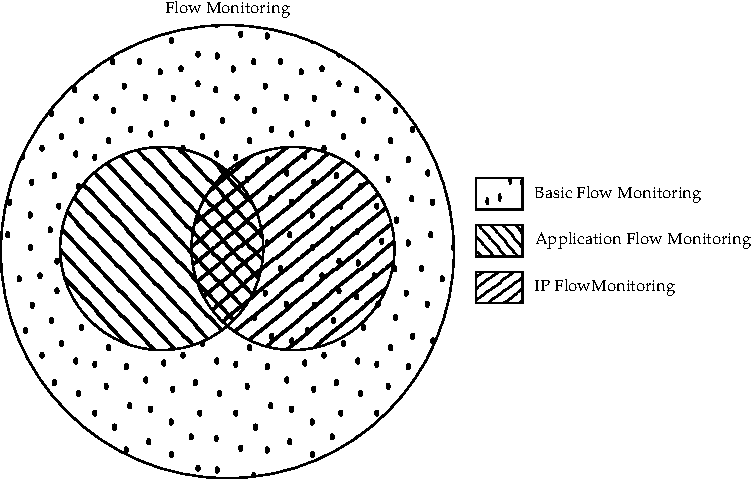
\includegraphics{figures/flow-monitoring-types}
  \end{center}
  \caption{Relations between Different Flow Monitoring Types}
  \label{fig:flow-monitoring-types}
\end{figure}

% explain that application flow monitoring means that:
% - primary: information from application layer is added to flow records
% - secondary:
%  - application logic (not necessarily in L7) affect the flow creation process, e.g. monitoring of tunnels
%  - less typical but can also be considered as application flow monitoring: additional information can be added to flow records from external sources (geolocation)

We have already stated that application flow monitoring is a flow monitoring that uses application information. Let us now consider how that information can be used for creating flows and flow records. Firstly, the goal is to provide application layer information in the flow records. Therefore the flow record needs to be extended with fields containing information extracted from the application layer of the packets of the flow. Secondly, an application logic can affect the flow creation process. For example, a flow with continuous HTTP connection can be split to multiple flows based on individual observed HTTP requests. Moreover, the application logic that affects flow creation is not be limited to application layer data, although the difference between basic flow monitoring and application flow monitoring is very thin in this case. Consider a scenario where Generic Routing Encapsulation (GRE) is used. As a basic flow, the GRE tunnel would be observed as a single flow. However, the GRE protocol can be considered an application and by using the semantics of this application, we can split the single flow to many flows based on the traffic that flows through the GRE tunnel. Thirdly, additional information can be inserted from external sources based on the semantics of properties extracted from the packets. For example, a geolocation information can be added to the flow records by the probe based on IP addresses of the communicating parties.

Now that the requirements for the application flow monitoring have been specified, we can formulate the application flow definition as follows:

\begin{definition}\label{def:application-flow}

    An \emph{\Index{application flow}} is a \emph{flow} where either
    the content of application layer or application logic is used
    to derive the flow keys.

\end{definition}

The definition specifies what an application flow is. Notice, however, that the definition does not cover all flows that are created by application flow monitoring. The problem is that the definition of application flow cannot specify how the subsequent flow record derived from the application flow will be created. For this reason, we need a definition of application flow record as well:

\begin{definition}\label{def:application-flow-record}

    An~\emph{\Index{application flow record}} is a \emph{flow record} 
    that contains information derived from either:

    \begin{enumerate}
        \item data contained in the application layer of the \emph{flow}, or
        \item external source of information.
    \end{enumerate}
        
\end{definition}

Application flow monitoring is a subset of flow monitoring where application flows or application flow records are used. Notice that application flow record can be created from standard flow record by extracting information from the application layer. Conversely, standard flow records can be created from application flows. Therefore, either the use of application flows or application flow records is enough to call the related monitoring process \emph{application flow monitoring}.

\section{Creating Application Flow}\label{sec:creating-application-flow}

Application flow monitoring significantly affects the whole flow monitoring process including the data processing on the collector. The most important impact is on the packet processing and flow creation processes of the flow exporter. The packet reception is not affected unless the packets are preprocessed in a hardware accelerated NIC. This section describes important features of application flow monitoring and their impact on the flow monitoring process.

\subsection{Packet Processing}

The primary goal of packet processing is to extract values of chosen properties of individual packets and packet treatment information. Packet processing in basic flow monitoring can be done using simple packet parsers. These packet parsers only need to be able to process packet headers with simple structures and the type of the following header is almost always determined by the content of the previous header. However, the type of application in the packet payload cannot usually be recognized from the packet headers. It is not necessary since every client must know where to connect and the server is expected to communicate only with clients using the correct protocol. Therefore, the flow exporters must identify the communicating applications themselves if they are to process the application payloads.

There three techniques that are used for application identification nowadays. The first and oldest one is based on well-known port numbers assigned and maintained by IANA~\cite{IANA-2017-Service}. Although this method is very simple, fast, and easily implemented, it is not very precise. Since one of the goals of flow monitoring is to provide reliable data for network security, it would be easy for malicious parties to use ephemeral port numbers for their activities to hide their traffic. Moreover, well-known port numbers are often changed legitimately by administrators to improve security. Although this practice is condemned as a case of ``security through obscurity'', it helps to mitigate a large number of attacks. The second, more reliable, method of application identification is signature based. The application data of each protocol often carry a specific header which can be recognized by pattern matching. Such headers are usually present in the first packets of the connection, therefore the identification happens early enough for the packet processing to be able to process the relevant application data. There are several application identification libraries and related sets of signatures. The paper by \citeauthor{Bujlow-2015-classification}~\cite{Bujlow-2015-classification} compares the performance of two commercial and four open-source traffic classification tools. Thirdly, machine learning can be used for application identification, as described in Section~\ref{sec:app-rel-work}. However, these methods often require features that are available only after the flow is exported, such as the number of packets or timing between individual packets. Since machine learning cannot usually recognize the application after first data packet, which often contains the most important information, it is not used for traffic classification by flow exporters.

We have already shown examples of aggregated and non-aggregated basic flow properties in Chapter~\ref{chap:network-flow-monitoring}. Properties extracted from application data are mostly aggregated as they are not present in every packet of the flow. Moreover, they are very often present only in a single packet of the flow, e.g. the properties found in HTTP header or parameters of TLS connection during the handshake. The aggregation function applied in such cases is \emph{firstOf}, which means that the first value of the property is used. 

Basic flow records are usually created from the first layers of the packets. The most common example is flow monitoring skipping the \emph{link layer} (e.g. Ethernet), extracting information from the \emph{network layer} (e.g. IPv4 or IPv6) and the \emph{transport layer} (e.g. TCP, UDP, ICMP). However, the protocol encapsulation can be much more complicated. For example, protocols such as IP in IP, Generic Routing Encapsulation (GRE), and PPTP allow to create virtual connections and provide a second layer of headers in each packet. Basic flow monitoring usually creates flows from the first layer it encounters. However, when the flow exporter searches for application layer, it should traverse all underlying layers as well. Moreover, the layer from which the flow records are created must be well defined. It is even possible to create flows based on higher layers and therefore split a single basic flow record based on its content. More details on this process are provided in Chapter~\ref{chap:traffic-analysis-using-application-flow-monitoring}.

The creation of application layer parsers is a complicated process. Although there are several tools designed for this purpose, as shown in Section~\ref{sec:app-rel-work}, it is often more efficient to create a particular parser from scratch. We have built several application parsers by hand and using lexical analysis tools for the HTTP protocol and evaluated their performance in Section~\ref{sec:http-parser-design}.

\subsection{Flow Creation}

\begin{figure}[t!]
  \begin{center}
    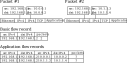
\includegraphics{figures/encapsulation}
  \end{center}
  \caption{Traffic Encapsulation Example}
  \label{fig:encapsulation}
\end{figure}

The flow creation process is affected in two ways. Firstly, properties derived from application values can be part of a flow key. This is the case of encapsulated protocol where the payload contains more IP headers, as shown in the Figure~\ref{fig:encapsulation}. If the addresses of the second IP header are used in flow keys, the basic flow is split into multiple flows, as described in the previous section. Secondly, the flows can be split when a certain application event occurs. The description of the second case follows.

Application protocol measurement may require flow record to be expired early. For example, when HTTP protocol supports pipelining, multiple requests and responses can be carried out over a single connection. When it is desirable to keep track of each request/response pair, existing flow record might be exported when a new request is encountered on the same connection. This is an example of the situation in which application logic affects the creation of flows, for which reason they become application flows. Note that the application flow monitoring may affect the number of generated flow records. This needs to be taken into consideration during further processing of the flow records.

To generalize the previous example, the application flow monitoring affects not only flow keys, but the flow expiration as well. Therefore, we add \emph{application event} to the existing flow expiration reasons (inactive timeout, active timeout, natural expiration, resource constraints, exporter termination). The application event expiration is usually implemented when the single connection is reused for multiple events of the same kind. Another example apart from the HTTP pipelining is FTP file transfer, where multiple files are transferred using a single connection, or SMTP connection where multiple messages are delivered at once.

The flow record values extracted from application layer are often present only in a single packet (e.g. HTTP header properties). This causes the information to be lost when the flow is long and an active timeout is triggered. The new flow record cannot contain the application information since it is not present anymore during its creation. There are two ways to solve this issue. The first is to do nothing during the flow creation and handle the problem during flow data processing. The previous flow records can be looked up and the necessary information can be extracted from them. The advantage of this method is that statistical queries about application layer data are not affected since the application data are always confined to a single record in this case. The second option is to copy the relevant application information to the new flow record upon active timeout. The information is then easily accessible during flow data processing, however, it is duplicated and special care needs to be taken when performing statistical queries on the flow data. Either of these options can be taken, but the flow data processing system must be aware of it.

A negative impact of the application flow monitoring on the flow creation process is the increased size of flow records. The information extracted from application protocols can be quite large in comparison to network and transport layers lengths. While the typical IPv4 header length is 20 bytes, typical TCP header length is 32 bytes, the HTTP URL can easily be several hundred bytes long. Therefore, the length of flow records of application flow monitoring is several times larger than without the application layer. There are two main negative impacts of such large flow records. Firstly, the flow cache might require much more RAM than basic flow monitoring flow cache. Secondly, even if the cache fits into RAM, it degrades the performance of the memory accesses because data locality is decreased and a CPU experiences more cache misses. For these reasons, it must be carefully considered which information is placed in each flow record and how it is encoded.

\subsection{Flow Export}

The flow export is affected by application flow monitoring in two ways. Due to the larger flow records the amount of exported data increases. The second is that when a template based protocol such as IPFIX is used, the number of templates increases fast with each new combination of supported protocols.

The most important thing that changes for flow export when flow monitoring is applied is that the flow records might be much longer. This can cause a congestion of the management link. When only a part of the data is necessary for flow processing on the collector, the exported data can be shortened. For example, only hostname and fixed length beginning of the URL can be exported for the HTTP protocol. However, since this leads to decreased quality of the exported data, information about the original data, such as original URL length, should be exported as well. The additional data allow the collector to correctly estimate the amount of missing information and apply the necessary algorithm to account for it. Long flow records also have a significant impact on flow record fragmentation when UDP protocol is used. Flow records longer than network interface MTU cannot fit into a single packet and must be fragmented, unless the transport protocol, such as TCP,  or flow export protocol handles fragmentation instead. The fragmentation puts additional load on flow collectors and causes increased data loss.

Exporters using template-based protocols, such as IPFIX, need to manage a significant number of templates when application flow monitoring is applied. This can cause performance issues since a template lookup needs to be performed for each flow record. Moreover, flow collectors need to process the templates as well. If the data are stored, for example, in a relational database and each template is represented by a table, a large number of tables can cause the queries to be slow since a union over many tables would need to be performed. Similar problems arise for other forms of flow storage and processing as well.


\section{Design of an HTTP Parser: A Study}\label{sec:http-parser-design}

It has been observed that the HTTP protocol became a ``new Transmission Control Protocol'' (TCP). More and more applications rely on HTTP protocol, e.g. Web 2.0 content, audio and video streaming, instant messaging etc. HTTP traffic (TCP port 80) can usually pass through most firewalls and therefore presents a standard way of transporting/tunnelling data. The versatility, ubiquity, and amount of HTTP traffic make it easy for an attacker to hide malicious activities. Missing application layer visibility renders standard NetFlow and IPFIX to be ineffective for HTTP monitoring.

The research presented in this section attempts to answer the following question: What are the impacts of application layer analysis of HTTP protocol on flow exporters and flow monitoring process? The contribution of our work in this section is threefold: Firstly, we have designed and evaluated several HTTP protocol parsers representing current state-of-the-art approaches used in today's flow exporters. Secondly, we have introduced a new flex-based HTTP parser. Thirdly, we report on the throughput decrease (performance implications of application parser) which is of the utmost importance for high-speed deployments.

The rest of this section is organized as follows. Subsection~\ref{subsec:http-related_work} describes related work. Subsection~\ref{subsec:http-tool_design} contains a description of the HTTP inspection algorithms and the framework that was used to test the algorithms. Subsection~\ref{subsec:http-metodology} describes the methodology used for HTTP parsers performance comparison. Subsection~\ref{subsec:http-perform_evaluation} presents the performance evaluation of the individual algorithms. Finally, Subsection~\ref{subsec:http-conclusion} contains our conclusions.

\subsection{Related Work} \label{subsec:http-related_work}

Application layer protocol parsers are an integral part of many network monitoring tools. We explored the source code of the following frameworks to see how the HTTP parsing is implemented. nProbe uses standard glibc~\cite{GNUProject-2017-GNU} functions like \emph{strncmp} (compare two strings) and \emph{strstr} (locate a substring). YAF uses Perl Compatible Regular Expressions (PCRE)~\cite{Hazel-2015-PCRE} to examine HTTP traffic. Suricata~\cite{OISF-2017-Suricata} and Snort~\cite{Roesch-1999-Snort} are both written in C. Suricata uses LibHTP~\cite{Qualys-2017-LibHTP} library which does HTTP parsing using custom string functions while Snort does its parsing using glibc functions. httpry~\cite{Bittel-2014-httpry} is another HTTP logging and information retrieval tool which is also written in C and uses its own built-in string functions. These HTTP parsers are hand-written.

Another approach is taken by Bro~\cite{Paxson-1999-Bro} authors. They use binpac~\cite{Pang-2006-binpac}, which is a declarative language and its compiler designed to simplify the task of constructing robust and efficient semantic analyzers for complex network protocols. They replaced some of Bro existing analyzers (handcrafted in C++) and demonstrated that the generated parsers are as efficient as carefully hand-written ones.

In this section, we try to determine whether these approaches to HTTP parsing can handle large traffic volumes. Besides the above approaches, we propose to use the Fast Lexical Analyzer (Flex)~\cite{Levine-2009-Flex} to design a new HTTP parser. Flex converts expressions into a lexical analyzer that is essentially a deterministic finite automaton that recognizes any of the patterns. The algorithm that converts a regular expression directly to deterministic finite automaton is described in \cite{Lesk-1975-Lex} and \cite{McNaughton-1960-Regular}.

There are other works that inspect the HTTP protocol headers. In~\cite{Schneider-2008-new} the authors use statistical flow analysis to differentiate traditional HTTP traffic and Web 2.0 applications. In~\cite{Torres-2012-Identifying} the authors identify HTTP sessions based on flow information. In both cases, a ground truth sample is needed, which is a topic addressed by~\cite{Torres-2012-Strategies}. In~\cite{Gehlen-2012-Uncovering} and \cite{Mahanti-2011-Characterizing} the authors use DPI to obtain information from the HTTP headers. Our approach is orthogonal to these works since we are interested in extending basic flow records with HTTP data.

\subsection{Parser Design} \label{subsec:http-tool_design}

HTTP protocol~\cite{rfc7230} has a number of properties that can be monitored and exported together with basic flow data. The most commonly monitored ones are present in almost every HTTP request or response header. Based on the properties monitored by the state-of-the-art DPI tools we selected the following ones for our parsers: \emph{HTTP method, status code, host, request URI, content type, user agent and referer}. Keeping track of every bidirectional HTTP connection is too resource consuming on high-speed networks, thus we focus on the evaluation of each individual packet. This approach is more common for flow exporters since it is more resistant to resource depletion attacks.

% This should be floating, but it is impossible to get labels straight when wrapped in figure env.
\noindent\hspace{1pt}
\begin{minipage}[t]{(0.49\textwidth)-2pt}
\begin{algorithm}[H]
\caption{\emph{strcmp} }
\label{alg:strcmp}
{\fontsize{8}{10}\selectfont
\begin{algorithmic}[1]
    \IF{first line contains ``HTTP''}
        \WHILE{\NOT end of HTTP header}
            \FOR{every parsed HTTP field}
                \IF{field matches the line}
                    \STATE{store the value of the line}
                \ENDIF
            \ENDFOR
            \STATE move to the next line
        \ENDWHILE
        \RETURN{HTTP packet}
    \ELSE 
        \RETURN{\NOT HTTP packet}
    \ENDIF
\end{algorithmic}
}
\end{algorithm}
\end{minipage}%
\hfill
\begin{minipage}[t]{0.47\textwidth}
\begin{algorithm}[H]
\caption{\emph{pcre}}
\label{alg:pcre}
{\fontsize{8}{10}\selectfont
\begin{algorithmic}[1]
    \IF{first line contains ``HTTP/x.y''}
        \FORALL{PCRE rules}
            \IF{rule matches}
                \STATE{store the matched value}
            \ENDIF
        \ENDFOR
        \RETURN{HTTP packet}
    \ELSE 
        \RETURN{\NOT HTTP packet}
    \ENDIF
\end{algorithmic}
}
\end{algorithm}
\end{minipage}
\vspace{10pt}

We implemented and evaluated three different types of parsing algorithms. The first algorithm (\emph{strcmp} approach) loops the HTTP header line by line and searches each line for given fields. It uses standard glibc string functions like \emph{memchr}, \emph{memmem} and \emph{strncmp}. The simplified pseudocode is shown in Algorithm~\ref{alg:strcmp}. The second algorithm (\emph{pcre} approach) uses several regular expressions taken from YAF to search the packet for specific patterns indicating HTTP header fields. The pseudocode for the \emph{pcre} algorithm is shown in Algorithm~\ref{alg:pcre}. We designed the third algorithm (\emph{flex} approach) to handle each packet as a long string. It uses finite automaton to find required HTTP fields and the Flex lexer is used to process the packets. The automaton design is shown in Fig.~\ref{fig:flex_schema}.

\begin{figure}[t]
        \centering
        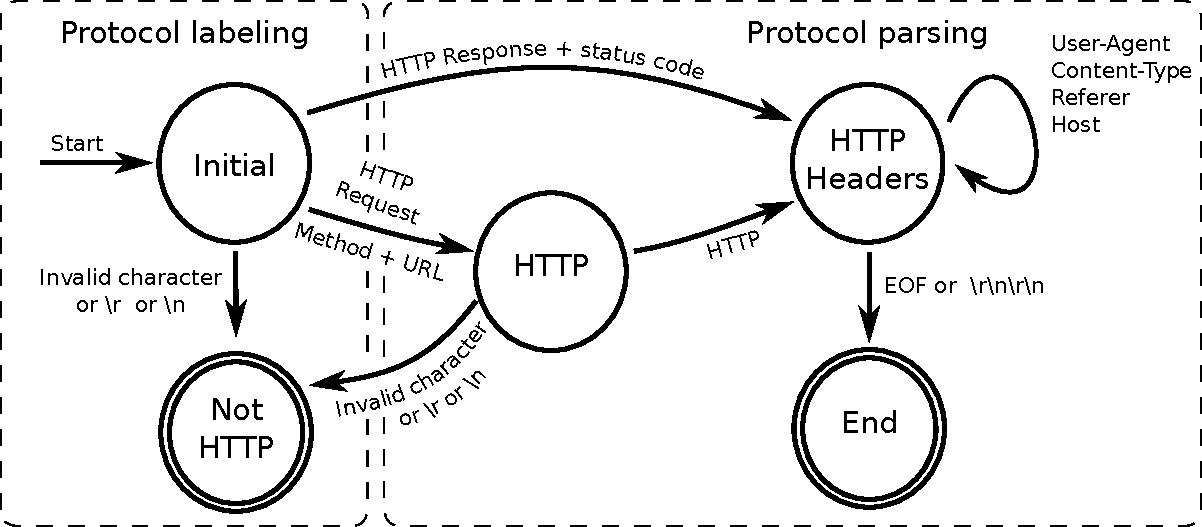
\includegraphics[width=0.8\textwidth]{figures/paper-http/flex_schema}
        \caption{\emph{flex} Algorithm Schema}
        \label{fig:flex_schema}
\end{figure}

Since the Flex is a generic tool, its initialization before scanning each packet is quite an expensive operation. Therefore we decided to remove all unnecessary dynamic memory allocations and costly initializations to see whether the performance can be increased. We named the new version \emph{optimized flex}. The disadvantage of Flex is that it has to keep the data in its own writeable buffer. Therefore the received data must be copied to such a buffer, which adds to the processing costs significantly. The advantage of the \emph{flex} parser is its simple maintenance and extension possibilities. The framework can be modified to parse any other application layer protocol just by changing the set of regular expression rules. The \emph{strcmp} parser would have to be rewritten from a scratch.

The \emph{strcmp} implementation also offers a space for further improvement. Algorithm~\ref{alg:optimized-strcmp} shows an \emph{optimized strcmp} version of the code that features a better processing logic. The optimized version searches for specific strings by comparing several bytes at once, which is done by casting the character pointer to integer pointer. The number that is compared to the string is computed from ASCII codes of the characters and converted to network byte order. The size of the used integer depends on the length of the string; longer integers offer better performance.

To focus only on the HTTP parsing algorithms we decided to let the FlowMon exporter~\cite{FlowmonNetworks--Flowmon} handle the packet preprocessing. We used a  benchmarking (input) plugin that reads packets from PCAP file to memory at start-up. Then it supplies the same data continuously for further processing. This approach allows us to focus on benchmarking the algorithms without the necessity of considering the disk I/O operations. We provide the source code of implemented algorithms and used packet traces at our homepage~\cite{Sima-2013-FlowMon}.

\begin{algorithm}[tb]
\caption{\emph{Optimized strcmp}}
\label{alg:optimized-strcmp}
{\fontsize{8}{10}\selectfont
\begin{algorithmic}[1]
    \IF{payload begins with ``HTTP''}
%       \STATE \COMMENT{HTTP response}
        \STATE store status code
        \WHILE{\NOT end of HTTP header}
            \FOR{every parsed response HTTP field}
                \IF{line starts with field name}
                    \STATE{store the value of the line}
                \ENDIF
            \ENDFOR
            \STATE move to the next line
        \ENDWHILE
        \RETURN{HTTP response packet}
    \ENDIF
    \IF{payload begins with one of GET, HEAD, POST, PUT,\\
            \hspace{\algorithmicindent}\hspace{\algorithmicindent}DELETE, TRACE, CONNECT}
%       \STATE \COMMENT{HTTP request}
        \STATE store request URI
        \WHILE{\NOT end of HTTP header}
            \FOR{every parsed request HTTP field}
                \IF{line starts with field name}
                    \STATE{store the value of the line}
                \ENDIF
            \ENDFOR
            \STATE move to the next line
        \ENDWHILE
        \RETURN{HTTP request packet}
    \ENDIF
    \RETURN{not HTTP packet}
\end{algorithmic}
}
\end{algorithm}

\subsection{Evaluation Methodology} \label{subsec:http-metodology}

In this section, we define a methodology of HTTP protocol parsers evaluation. We focus on parsing performance (number of processed packets per second) of the algorithms described in Section \ref{subsec:http-tool_design} from several different perspectives.

The first perspective focuses on the performance comparison with respect to analyzed traffic structure. The second perspective covers the impact of the number of HTTP fields supported by the parser. The third perspective describes the effect of a Carriage Return (CR or \verb!'\r'!) and a Line Feed  (LF or \verb!'\n'!) control characters distribution in the packet payload.

A common technique of increasing network data processing performance is processing only important part of each packet. Therefore, we perform each of the tests in two configurations. In the first configuration, the parsers are given whole packets. This is achieved by setting the limit on packet size to 1500 bytes, which is the most common maximum transmission unit value on most Ethernet networks. In the second configuration the parsers are provided with truncated packets of length 384 bytes, which is the minimum packet length recommended for DPI by authors of the YAF exporter~\cite{Inacio-2010-YAF}.

To test the performance of the parsers, we created an HTTP traffic trace (testing data set). Our requirements on the data set were as follows: preserve the characteristics of HTTP protocol, reflect various HTTP traffic structures and have no side effects on the flow exporter. In order to meet these requirements, we decided to create a synthetic trace.

The HTTP protocol is a request/response protocol. To preserve the characteristics of HTTP protocol during the testing a random request, response and binary payload packet were captured from the network. To omit the undesirable bias of the measurement only these three packets were used to synthesize test trace. The final test trace consists of 200 packets. In order to reflect various traffic structures, we suggested following ratio:

\begin{align}
       r = \frac{\# \text{request packets}+\#\text{response packets}}{\#\text{all packets}}*100
\end{align}

where $r \in [\,0,100\,]$ and created a test set for each integer ratio from the interval. Further, we created two packets with the modified payload. One packet contained the CR and LF control characters only at the very \emph{beginning} of the packet payload, the other one only at the \emph{end}. For both of the modified packets and for the \emph{unchanged} packet the test trace for each integer ratio was created.

% Network analysis tools trim the packets in order to increase throughput. However, we should set the trim limit to the smallest number that will capture the HTTP information, we are interested in. We investigate the influence of the trim value on the performance, thus we select two limits. In the first case, we set the limit to 1500\,B which refers to the standard Ethernet frame length. In the other case, we set the limit to 384\,B which is recommended by YAF as a minimum payload length for the best results \cite{Inacio-2010-YAF}.

Having defined the test trace, we propose the following case studies to cover all evaluation perspectives. The case studies are carried out for both full and truncated packets. Moreover, we measure the performance of the flow exporter without an HTTP parser (\emph{no HTTP} parser). This way we can estimate the performance decline caused by increased application layer visibility.

\begin{enumerate}
    \item \emph{Performance Comparison}: This case study compares the parsing performance of implemented parsers. Moreover, we report on the flow exporter performance without an HTTP parser (\emph{no HTTP} parser).
    \item \emph{Parsed HTTP Fields Impact}: This case study shows a parser performance with respect to the number of supported HTTP fields. We incrementally add support for new HTTP fields and observe the impact on the parser performance.
    \item \emph{Packet Content Effect}: The result of this study presents the influence of the CR and LF control characters position in a packet payload on the parser performance. The test traces containing modified payload packets are used to perform the measurement.
\end{enumerate}

The performance evaluation process employs the benchmarking input plugin (see Subsection~\ref{subsec:http-tool_design}) to obtain the number of processed packets per second. 
In order to avoid influencing the results, the plugin uses a separate thread and CPU core for the accounting. The plugin counts the number of the processed packets in ten-second interval and then computes the packets per second rate. We have operated the benchmark plugin for fifty seconds for each test trace and computed a number of packets processed and a standard error of the measurement. The parsed HTTP header fields impact and packet content effect were assessed in a similar way. All measurements were conducted on a server with the following configuration: Intel Xeon E5410 CPU at 2.33\,GHz, 12\,GB 667\,MHz DDR2 RAM and Linux kernel 2.6.32 (64 bit).

\subsection{Parser Evaluation} \label{subsec:http-perform_evaluation}

In this section, we present results of HTTP parser evaluation. First, we describe the parser performance comparison, then we investigate the impact of supported HTTP header fields. Finally, the effect of the packet content on HTTP parsing performance is shown.

\subsubsection*{Performance Comparison.}

This case study uses the standard version of each parser that supports seven HTTP fields. The data set containing the unmodified payload packets is used and the parsers are tested both on full and truncated packets. Fig.~\ref{fig:http-pcap_1500} shows the result for full packets case study and Fig.~\ref{fig:http-pcap_384} shows performance evaluation for truncated packets.

First we discuss the Fig.~\ref{fig:http-pcap_1500}. The \emph{no HTTP} meter is capable of parsing more than 11 million packets per second. This result is not influenced by the application data carried in the packet since the data is not accessed by the \emph{no HTTP} parser. Employing event the fastest of the HTTP parsing algorithms the performance drops to the nearly one half of parsed packets per second. All of the HTTP parsers show the decrease in the performance as the ratio $r$ increases since the amount of request and response packets, which are more time demanding to parse, grows.

\begin{figure}[tb]
        \centering
        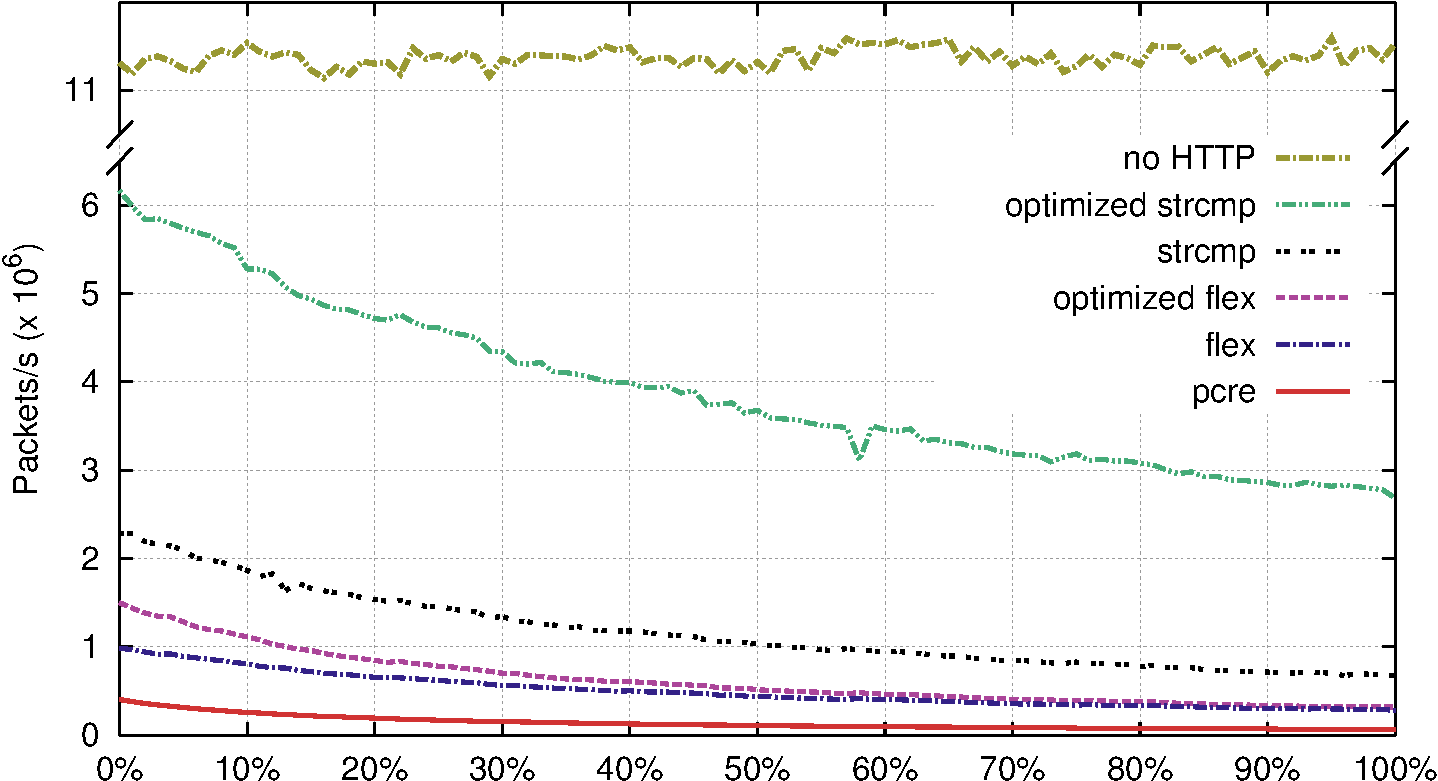
\includegraphics[width=0.8\textwidth]{figures/paper-http/1500_pcap_norm_1}
        \caption{Parser Performance Comparison with Respect to HTTP Proportion (0\,\% - No HTTP, 100\,\% - Only HTTP Headers) in the Traffic - Full Packets 1500\,B.}
        \label{fig:http-pcap_1500}
\end{figure}

The best performance is achieved by \emph{optimized strcmp} parser, which uses application protocol and code level optimizations. The parser takes into account the HTTP header structure, the difference between HTTP request and response headers and looks only for header fields that can be found in the specific header type. The code level optimizations include converting static strings into integers and matching them against several characters at once, which can be done in one processor instruction. The \emph{strcmp} parser performance is the second best, although the throughput is less than half of the \emph{optimized strcmp} parser.

The main difference between \emph{flex} and \emph{optimized flex} parsers is in the automaton initialization process. By rewriting the initialization process we achieved slight performance improvement, which is noticeable mainly in the $\langle\,0\,\%,20\,\%\,\rangle$ interval, where the actual HTTP parsing time is short. There is one other important factor affecting the \emph{flex} parser performance. The flex automaton is designed to work with its own writable buffer since it marks the end of individual parsed tokens directly into the buffer. For this reason, a copy of the packet payload must be created before the actual parsing can start. To measure the impact of the copying, we created another two parser plugins called \emph{empty} and \emph{copy}. First, we measured the flow exporter throughput with \emph{empty} plugin which performs no data parsing, then with \emph{copy} plugin which only copies packet payload to a static buffer. From the results, we estimate the throughput the \emph{optimized flex} parser would have without the memory copying. The performance of the \emph{optimized flex} parser would be about 2.4\,million packets per second for 0\,\% and 0.33\,million packets per second for 100\,\% HTTP packets. This shows that the actual HTTP parsing when compared to \emph{strcmp} parser, is slightly faster for binary payload packets and slower for HTTP header packets.

The performance of the \emph{pcre} parser is the lowest. The PCRE algorithm converts the regular expression to a tree structure and then performs a depth-first search while reading the input string. In case there is no match in the current tree branch, the algorithm backs up and tries another one. Therefore, for a complex regular expression, the pattern matching is not that fast as simple string search using functions like \emph{strcmp}. Another reason why the \emph{pcre} parser is not fast is that it performs all searches on whole packet payload. The other algorithms are processing the data sequentially.

\begin{figure}[tb]
        \centering
        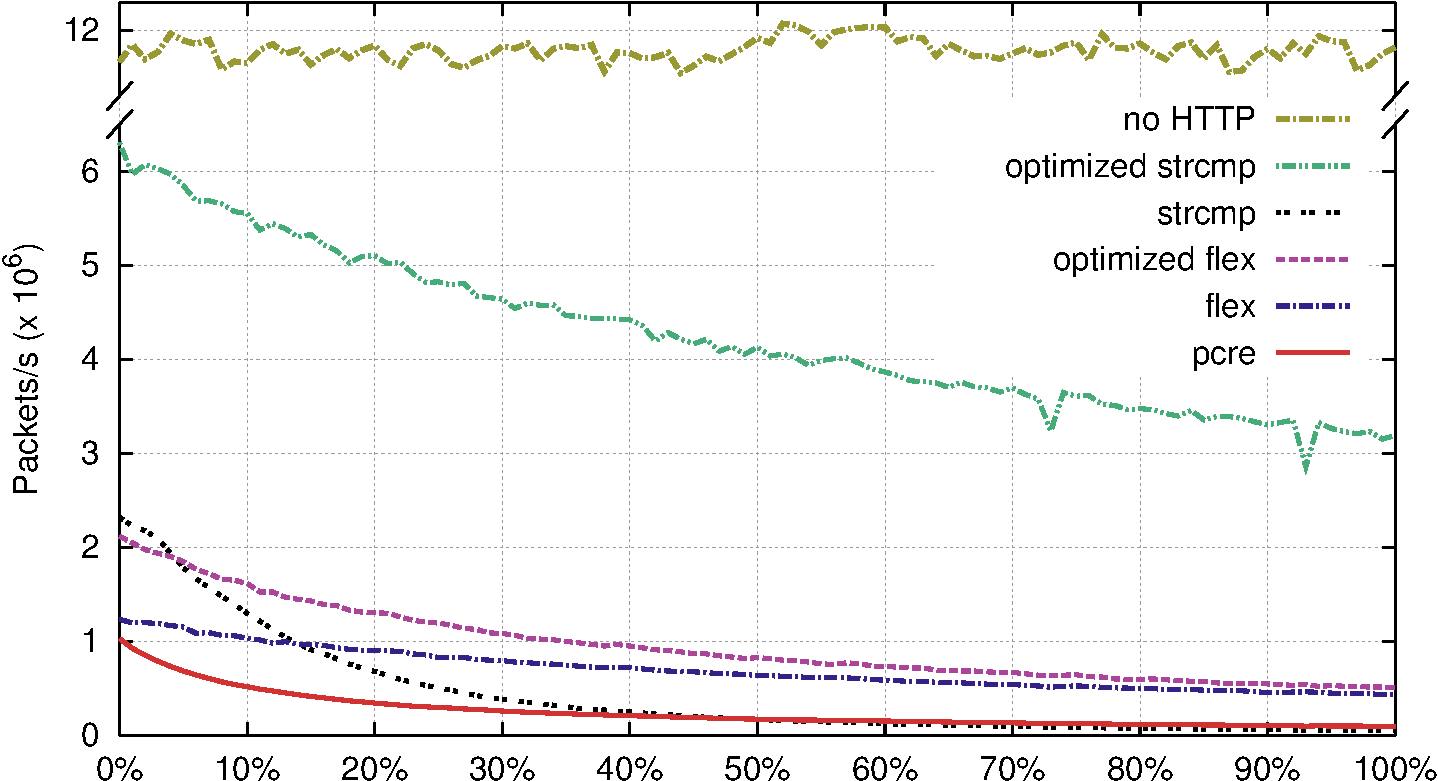
\includegraphics[width=0.8\textwidth]{figures/paper-http/384_pcap_norm_1}
        \caption{Parser Performance Comparison with Respect to HTTP Proportion (0\,\% - No HTTP, 100\,\% - Only HTTP Headers) in the Traffic - Truncated Packets 384\,B.}
        \label{fig:http-pcap_384}
\end{figure}

Fig.~\ref{fig:http-pcap_384} shows the results for truncated packets. The \emph{optimized strcmp} and \emph{no HTTP} are only slightly faster since the truncating of the packets has a positive impact on CPU data cache utilization. The \emph{strcmp} algorithm is flawed since its throughput on HTTP packets deteriorates rapidly. This shows the disadvantage of hand-written parsers, as they are more error-prone than the generated ones. The \emph{pcre} parser performance is almost doubled, as the repeatedly processed data are truncated. Flex based parser also achieve performance increase, since the memory copying costs are reduced for smaller data.

\subsubsection*{Parsed HTTP Header Fields Impact.}

This case study was designed to show the impact of a number of parsed HTTP header fields on the parser performance. 

When payload packets are detected, they do not have their content parsed for additional HTTP header fields. Therefore, a test set containing only HTTP request and response packets was used. The case study starts with an empty plugin, that does not parse HTTP header fields and just labels the HTTP packets. In the next steps, we cumulatively add an additional header field to parse until we parse all of the seven supported fields. We run the tests for both full and truncated packets. The average performance of the parsers for each of the added field is shown in Fig.~\ref{fig:http-field}.

\begin{figure}[tb]
    \centering
    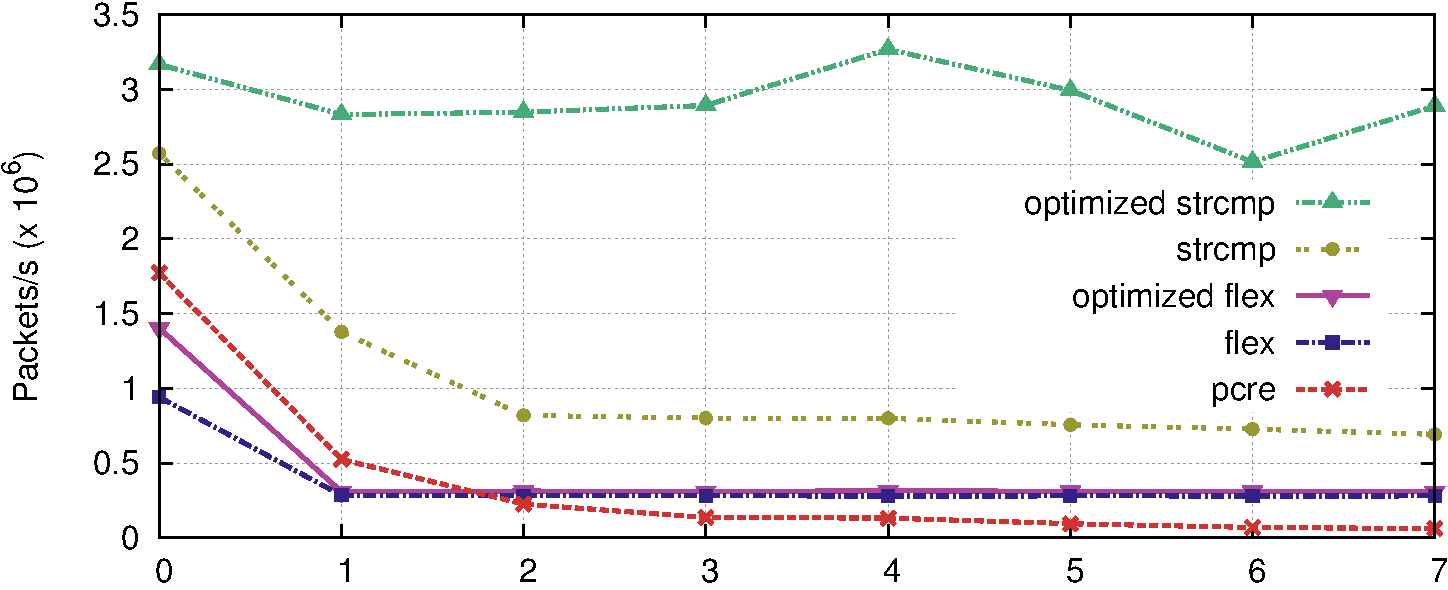
\includegraphics[width=0.8\textwidth]{figures/paper-http/mod_1500}
    \caption{An HTTP Parser Throughput for 1500\,B Packets; Supported Fields - (0) \emph{none} - HTTP Protocol labeling, (1) \emph{+host}, (2) \emph{+method}, (3) \emph{+status code}, (4) \emph{+request URI}, (5) \emph{+content type}, (6) \emph{+referer}, (7) \emph{+user agent}.} 
    \label{fig:http-field}
\end{figure}


Only the request and response packets are parsed, thus the values for the seven fields parsed in the Fig.~\ref{fig:http-field} correspond to the 100\,\% packet/s values in the Fig.~\ref{fig:http-pcap_1500} and Fig.~\ref{fig:http-pcap_384}. For the same reason the parsed packets per second numbers are lower in comparison with the Fig.~\ref{fig:http-pcap_1500} and Fig.~\ref{fig:http-pcap_384}. The performance of \emph{strcmp} and \emph{pcre} parsers drops with each additional parsed HTTP header field. The \emph{optimized strcmp} parser implementation details attentional fluctuation affect on performance shown in Fig.~\ref{fig:http-field}. An example is the performance increase when adding a \emph{(4) request URI} or a \emph{(3) status code}. It is caused by extra code snippet that extracts the URI so that this line is not processed by the more generic code designed for parsing other header fields. Due to the usage of the finite automaton, the data is always processed in one pass by the flex-based algorithms. Therefore, they retain the same level of performance for all additional fields. This feature could be used to automatically build powerful parsers when a large number of parsed application fields would make it ineffective to create hand-written parsers.

Same as in the previous case study, the parsers processing truncated packets show better performance than the parsers working on full packets.

\subsubsection*{Packet Content Effect.}

This case study investigates the possible effects of the position of the CR and LF control characters in the packet payload on the parser performance. The mentioned ASCII characters represent the end of line in the HTTP header. Some of the proposed algorithms use these characters as the trigger to stop parsing. Therefore the position of these characters affects the performance of the parsers. The packets with the CRLF characters at the very \emph{beginning} should be parsed faster than the packets having the CRLF at the \emph{end} since the algorithm terminates as soon as it identifies the CRLF characters. The test sets with modified binary payload packets (see Subsection~\ref{subsec:http-metodology}) enables us to compare the algorithms taking into account this perspective.

\begin{figure}[t]
    \centering
    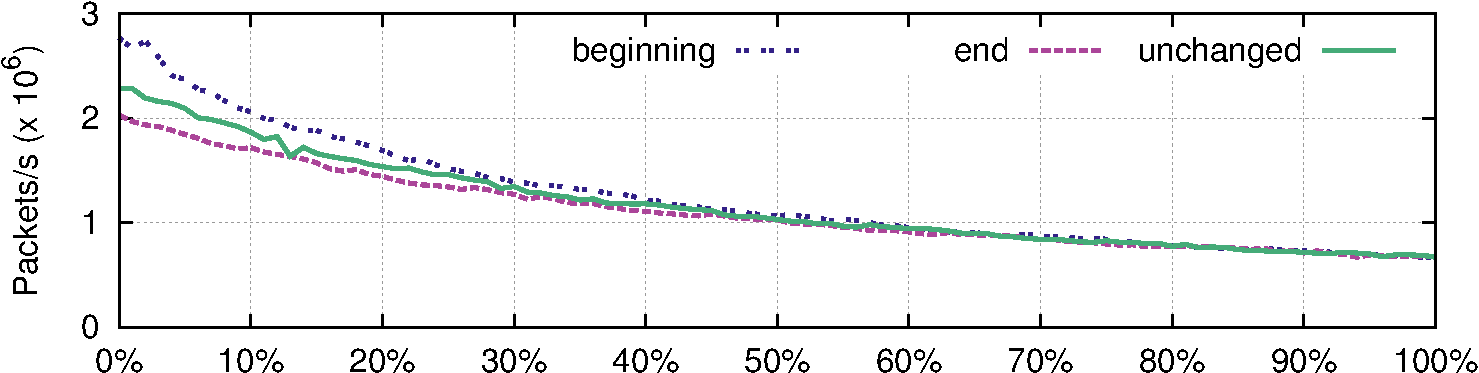
\includegraphics[width=0.8\textwidth]{figures/paper-http/1500_noflex}
    \caption{Packet Content Effect - Packet Length 1500\,B}
    \label{fig:http-packet_structure}
\end{figure}

We used the modified binary payload packets to test the parsers. The parsing algorithms, except the \emph{strcmp} algorithm, show an insignificant difference in their performance for all variants of the modified packets. The \emph{pcre} and \emph{optimized strcmp} parsers do not search for the end of line characters in order to label the packet, therefore this test does not affect them. The flex-based algorithms are not significantly affected since they stop parsing on the first character that is not expected in HTTP header and therefore stop at the first character in any case. The \emph{strcmp} parser depends on the search for end of line characters, which is confirmed by Fig.~\ref{fig:http-packet_structure}. The sooner the characters are found, the faster the algorithm terminates. The scenario with truncated packets is different since the performance on \emph{end} data set is greater than on \emph{unchanged} data. This is caused by removing the end of packet payload together with the end of line character. When the \
\emph{strcmp} algorithm cannot find the character, it terminates immediately without trying to search the data. Therefore it terminates sooner than on \emph{unchanged} data set, where the end of line character is found and the search continues.

\subsection{Conclusions} \label{subsec:http-conclusion}

This section has assessed the impacts of HTTP protocol analysis on flow monitoring performance. We implemented the state-of-the-art approaches to HTTP protocol parsing. Moreover, the new flex-based HTTP parser was designed and its performance was compared to the other approaches.

The evaluation shows that in our case the hand-written and carefully optimized parser performs significantly better than implementations with automated parsing. It also shows that the new flex-based implementations handle the increasing number of parsed HTTP fields without significant performance loss. Truncating the packets prior to HTTP protocol parsing can increase the parser throughput. The performance comparison of \emph{no HTTP} parser with HTTP parsers shows that providing an application visibility is a demanding task. Current approaches to the application protocol parsing may not be effective enough to process a high-speed network traffic.

Although we focused on HTTP header parsing in this section, measuring the overall performance of flow exporters is also essential. We will address performance evaluation and runtime requirements of entire flow exporter frameworks in our future work. This research will allow us to compare existing frameworks and new prototypes under equal conditions. Monitoring of HTTP application protocol exposes new challenges for flow exporters. In particular, an increased number of exported fields, large flow record length and their impact on transport protocol requires further research.


\section{Summary}\label{sec:app-summary}

This chapter has described the aspects of extending flow monitoring by using information from the application layer. We have argued that application monitoring is necessary to provide information about current network-based cybersecurity threats. Without the application insight, attackers can perform application layer attacks that have no impact visible using the basic flow monitoring. Therefore the application flow monitoring utilizes aspects of DPI to provide more fine-grained information about the observed traffic. 

We have briefly surveyed the state of the art of the application parsers creation process. There are several approaches that allow creating application parsers from a higher level description, which allows creating more robust and error-prone parsers. However, existing application flow exporters do not often use these approaches and implement their own application parsers. Moreover, although most flow exporters support application identification, only a few of them provide real application visibility. 

The existing sources do not use consistent terminology regarding the application flow monitoring. Therefore, we have proposed a workable terminology that captures the current state of the art in the application flow monitoring. We call the flow monitoring without processing the application layer \emph{basic flow monitoring} and differentiate between \emph{IP flow monitoring} which is a term used for any flow monitoring that uses information from the IP layer. We have provided definitions of both \emph{application flow} and \emph{application flow record} and explained their relation to the flow and flow record definitions provided in Chapter~\ref{chap:network-flow-monitoring}.

Once the terminology of application flow has been established, we ventured to describe the application flow monitoring process, particularly the changes that it introduced to the general flow monitoring process described in the previous chapter. It impacts the flow creation on two main levels. Firstly, a new flow expiration reason has been introduced that can be triggered due to an application event. Secondly, the flow records became application flow records as they contain information from the application layer. These changes have an impact on the number of generated flow records as well as on their sizes.

The last contribution of this chapter is a description of a design of an HTTP protocol parser. We have shown several approaches to the construction of the parser, implemented them and evaluated their performance. We have quantified the flow monitoring performance drop caused by each of them and showed, that a hand-crafted parser can be highly optimized to provide the best throughput, although it requires much more expert programmer to implement it correctly.

